\chapter{运动与身体的能量需求}\label{ch:g10:exercise-and-energy}

一名骑车者在实验室自行车上蹬踏，对抗一个用来测量
她输出功率的制动器：\qty{100}{W}，然后\qty{150}{W}，再到\qty{200}{W}。
她脸上的面罩把每次呼吸都送入分析仪。屏幕上的数字
随制动器同步攀升：她输出的机械功越多，
耗氧量越大，呼出的二氧化碳也越多。她的肌肉
正以满负荷进行
\cref{ch:g10:cell-metabolism}中所述的呼吸作用，而分析仪
读取的正是这笔能量收支的账目。本章追踪运动中的能量，
从为其提供能量的食物，到释放能量的氧气。

\section{能量输入，功输出}

\begin{definition}[能量消耗]\label{def:g10:exercise-and-energy:expenditure}
人体的\emph{能量消耗}\index{能量消耗}，
以焦耳计，是其\omterm{def:g10:cells-common-unit:cell}{细胞}在给定时间内
从有机分子中释放的全部能量。除以时间，便是一个
\emph{\omterm{def:g10:cell-metabolism:metabolism}{代谢}功率}，以瓦特计。静息时，成年人约消耗
\qty{80}{W}——每天约 \qty{7000}{kJ}——用以维持心脏跳动、
大脑工作、体温保持在 \qty{37}{\celsius} 以及\omterm{def:g10:cells-common-unit:cell}{细胞}存活，
这便是\emph{基础\omterm{def:g10:cell-metabolism:metabolism}{代谢}}。每项活动
都会在此基础上增加消耗。
\end{definition}

\begin{proposition}[能量去向]\label{prop:g10:exercise-and-energy:efficiency}
工作中的肌肉只能将其释放的能量中约四分之一
转化为机械功，其余四分之三以热量形式散失。
因此，输出机械功率 $P$ 时，身体在静息水平之上
约需承担 $4P$ 的\omterm{def:g10:cell-metabolism:metabolism}{代谢}功率：骑车者以 \qty{100}{W} 蹬踏时，
她的肌肉中正消耗约 \qty{400}{W}，身体必须散去
\qty{300}{W} 的热量——主要靠出汗。
\end{proposition}
\admitted

\begin{example}[每日能量预算]\label{ex:g10:exercise-and-energy:budgets}
一名学生上课、步行上学和睡觉时，一天约消耗
\qty{9000}{kJ}；一小时足球运动额外增加约
\qty{2500}{kJ}；背着行囊在山中度过的一天，全天共
\qty{15000}{kJ}。一名骑车者在山地赛段中消耗 \qty{25000}{kJ}，
白天的进食无法补足这些消耗。能量来自食物
（见\cref{ch:g10:chemistry-of-life}）：每克\omterm{def:g10:chemistry-of-life:families}{糖类}或\omterm{def:g10:chemistry-of-life:families}{蛋白质} \qty{17}{kJ}，
每克\omterm{def:g10:chemistry-of-life:families}{脂质} \qty{38}{kJ}。
\end{example}

\section{耗氧量测量能量消耗}

\begin{proposition}[氧当量]\label{prop:g10:exercise-and-energy:oxygen}
由于运动中的能量由\omterm{prop:g10:cell-metabolism:respiration}{细胞呼吸}释放，
而\omterm{prop:g10:cell-metabolism:respiration}{细胞呼吸}要消耗氧气，因此人体的耗氧量可以测量其
\omterm{def:g10:exercise-and-energy:expenditure}{能量消耗}：每消耗一升氧气，对应
约释放 \qty{20}{kJ} 的能量，无论葡萄糖与\omterm{def:g10:chemistry-of-life:families}{脂质}如何混合燃烧。
静息时，人每分钟约消耗 \qty{0.25}{L}
氧气；运动时，耗氧量随输出功率成比例上升，
直至达到个人的上限。
\end{proposition}
\begin{proof}[依据]
由\cref{ch:g10:cell-metabolism}中的呼吸方程式可得，
\qty{2870}{kJ} 对应 \qty{6}{mol} 氧气，即每摩尔 \qty{478}{kJ}，
而一摩尔气体约占 \qty{24}{L}：每升约 \qty{20}{kJ}。
\omterm{def:g10:chemistry-of-life:families}{脂质}的数值为 \qty{19.6}{kJ/L}，\omterm{def:g10:chemistry-of-life:families}{糖类}为
\qty{21.1}{kJ/L}，因此混合比例影响甚微。
在密闭舱中进行的测量，直接收集受试者释放的热量，
其结果与氧气推算值相符，误差在百分之几以内。
\end{proof}

\begin{omfigure}
\begin{tikzpicture}
\begin{axis}[
  width=0.86\linewidth, height=5.8cm,
  axis x line=bottom, axis y line=left,
  xmin=0, xmax=320, ymin=0, ymax=4.2,
  xlabel={机械功率 (W)}, ylabel={$\mathrm{O_2}$ 消耗量 (L/min)},
  xlabel style={font=\small, at={(axis description cs:0.5,-0.12)}, anchor=north},
  ylabel style={font=\small},
  tick label style={font=\small},
  xtick={0,50,100,150,200,250,300}, ytick={0,1,2,3,4},
  clip=false,
]
\addplot[thick, omThm, mark=*, mark size=1.6pt] coordinates
  {(0,0.3) (50,0.9) (100,1.5) (150,2.1) (200,2.7) (250,3.2) (300,3.3)};
\draw[dashed, gray] (axis cs:0,3.3) -- (axis cs:320,3.3);
\node[font=\small, anchor=south east] at (axis cs:318,3.32) {$\dot V\!\mathrm{O_2}$max};
\node[font=\small, anchor=south west, align=left] at (axis cs:40,3.42) {斜率：每分钟 \qty{12}{mL} 的 $\mathrm{O_2}$\\ 每瓦};
\end{axis}
\end{tikzpicture}

{\small 受试者蹬踏、功率递增时的耗氧量。
耗氧量随功率线性上升——每瓦每分钟约 \qty{12}{mL} 氧气，
直至耗氧量达到上限，即受试者的
$\dot V\!\mathrm{O_2}$max；超过此值后，额外功率
靠无氧方式供给，且无法持续。}
\end{omfigure}

\begin{definition}[最大摄氧量]\label{def:g10:exercise-and-energy:vo2max}
称\emph{最大摄氧量}\index{最大摄氧量}
（记为 $\dot V\!\mathrm{O_2}$max），是人体能够摄取并
利用氧气的最高速率，以升每分钟计——或为比较不同体型的人，
以毫升每分钟每千克体质量计。
它决定了仅靠呼吸作用就能维持的最高功率。
典型值：久坐的成年人约 \qty{35}{mL/min}（每千克），
受训学生为 \num{50}，
优秀耐力运动员为 \num{80} 或更高。
\end{definition}

\begin{example}[读取曲线]\label{ex:g10:exercise-and-energy:reading}
由图可见，\qty{100}{W} 的蹬踏耗氧 \qty{1.5}{L/min}，
$1.5 \times 20 = \qty{30}{kJ}$，即每分钟
\qty{500}{W} 的\omterm{def:g10:cell-metabolism:metabolism}{代谢}功率——\qty{100}{W} 的机械功加上
\qty{400}{W} 的热量及静息需求，与
\cref{prop:g10:exercise-and-energy:efficiency}相符。该受试者的耗氧上限
为 \qty{3.3}{L/min}（体重 \qty{66}{kg}），
约合每千克 \qty{50}{mL/min}。
\end{example}

\begin{omfigure}
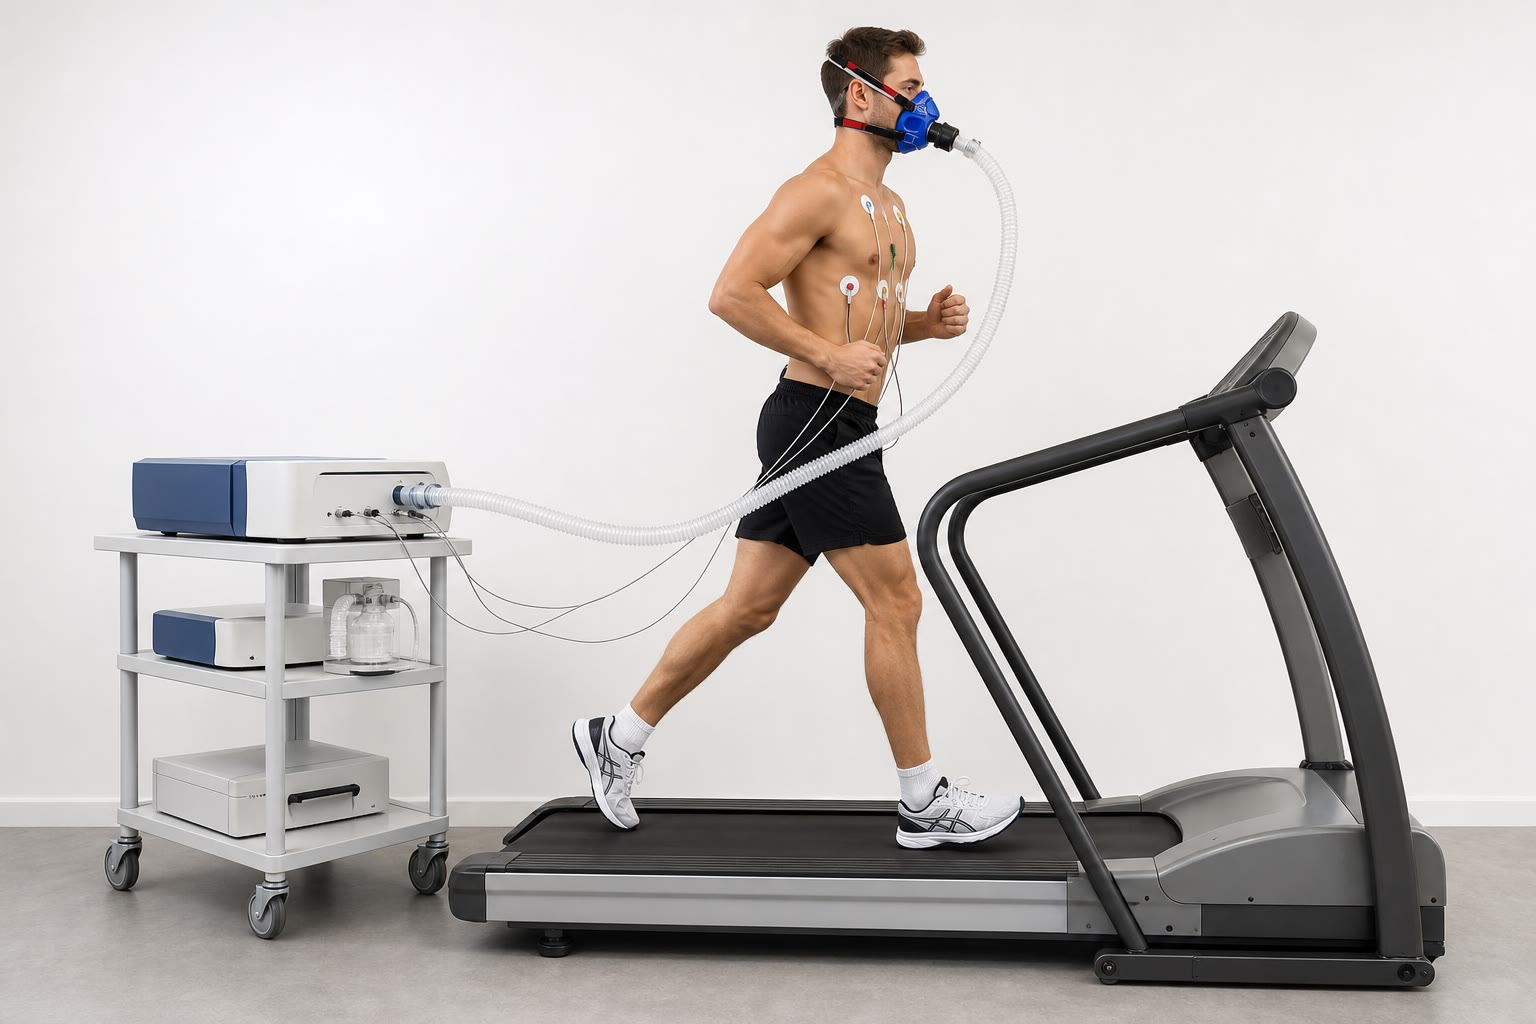
\includegraphics[width=0.62\linewidth]{images/book2/ai/g10-exercise-treadmill-mask.jpg}

{\small 运动时测量耗氧量：每次呼吸
经面罩送入气体分析仪，
逐分钟记录摄入的氧气和呼出的二氧化碳，同时
跑步机设定功率。}
\end{omfigure}

\section{肌肉的燃料}

\begin{proposition}[ATP 的三个来源]\label{prop:g10:exercise-and-energy:fuels}
肌肉收缩靠 ATP 供能，\omterm{def:g10:cells-common-unit:cell}{细胞}内的 ATP 只够
几秒钟的量。ATP 有三条补充途径，各有
自己的速率和容量：
\begin{itemize}
  \item 肌肉中少量的磷酸化合物储备，
        可立即重新生成 ATP，但只能维持约 10 秒，即
        短跑；
  \item \omterm{def:g10:cells-common-unit:cell}{细胞质}中葡萄糖的乳酸\omterm{def:g10:cell-metabolism:fermentation}{发酵}，速度快但
        效率低，可维持全力运动 1 至 2 分钟，
        并产生乳酸；
  \item \omterm{def:g10:cells-common-unit:organelle}{线粒体}中的\omterm{prop:g10:cell-metabolism:respiration}{细胞呼吸}，达到满速率较慢，
        但持续时间几乎不受限制，燃烧血液中的葡萄糖，
        肌肉中的\omterm{def:g10:exercise-and-energy:glycogen}{糖原}，以及
        体脂中的脂肪酸。
\end{itemize}
各途径所占的比例取决于
运动的强度与持续时间。
\end{proposition}
\admitted

\begin{omfigure}
\begin{tikzpicture}
\begin{axis}[
  ybar stacked, bar width=18pt,
  width=0.86\linewidth, height=5.6cm,
  axis x line=bottom, axis y line=left,
  ymin=0, ymax=100, ylabel={能量占比（\%）}, ylabel style={font=\small},
  symbolic x coords={10 s, 1 min, 4 min, 30 min, 2 h},
  xtick=data, xticklabels={10 秒, 1 分钟, 4 分钟, 30 分钟, 2 小时}, tick label style={font=\small},
  xlabel={全力运动的持续时间},
  xlabel style={font=\small, at={(axis description cs:0.5,-0.12)}, anchor=north},
  enlarge x limits=0.15,
  legend style={at={(0.5,-0.3)}, anchor=north, legend columns=3,
                font=\small, draw=none},
]
\addplot[fill=omThm!50, draw=omThm] coordinates {(10 s,85) (1 min,25) (4 min,8) (30 min,2) (2 h,1)};
\addplot[fill=omProp!50, draw=omProp] coordinates {(10 s,12) (1 min,50) (4 min,32) (30 min,8) (2 h,2)};
\addplot[fill=omDef!50, draw=omDef] coordinates {(10 s,3) (1 min,25) (4 min,60) (30 min,90) (2 h,97)};
\legend{磷酸化合物储备, 乳酸发酵, 细胞呼吸}
\end{axis}
\end{tikzpicture}

{\small 全力运动时三种 ATP 来源的大致占比，
随运动持续时间而定。100 米短跑主要依靠磷酸化合物储备；
400 米赛跑主要依靠乳酸\omterm{def:g10:cell-metabolism:fermentation}{发酵}；持续几分钟以上的运动主要依靠
\omterm{prop:g10:cell-metabolism:respiration}{细胞呼吸}。}
\end{omfigure}

\begin{definition}[糖原]\label{def:g10:exercise-and-energy:glycogen}
\emph{糖原}\index{糖原}是动物体内储存\omterm{def:g10:chemistry-of-life:families}{糖类}的形式：
由葡萄糖单元连接成的带支链长链，以颗粒形式
存在于肌肉\omterm{def:g10:cells-common-unit:cell}{细胞}（成人约 \qty{400}{g}）和肝脏（约 \qty{100}{g}）中。
肌糖原为储存它的肌肉供能；
肝糖原分解为葡萄糖释入血液，
使血糖维持在约 \qty{1}{g/L}，供脑和
其他组织利用。脂肪储存于脂肪\omterm{def:g10:cells-common-unit:cell}{细胞}中，是远为庞大的能源储备
（见\cref{ch:g10:chemistry-of-life}），但只能缓慢燃烧，
且须有氧气参与。
\end{definition}

\begin{example}[马拉松“撞墙”]\label{ex:g10:exercise-and-energy:wall}
跑步每千克体重每千米约耗能 \qty{4}{kJ}；
体重 \qty{70}{kg} 的跑者每千米耗能 \qty{280}{kJ/km}，
一场马拉松共耗能 \qty{11800}{kJ}。\omterm{def:g10:exercise-and-energy:glycogen}{糖原}储备约可提供
\qty{8500}{kJ}。若跑者消耗\omterm{def:g10:exercise-and-energy:glycogen}{糖原}过快，储备
会在约第 30 千米处耗尽；此后肌肉只能依靠脂肪供能，
而脂肪的供能速率几乎只有一半，配速随之骤降，
——即“撞墙”。训练有素的跑者一开始就
燃烧占比更大的脂肪，并在比赛中补充\omterm{def:g10:chemistry-of-life:families}{糖类}。
\end{example}

\begin{omfigure}
\begin{tikzpicture}[>=Stealth, font=\small,
  b/.style={draw, rounded corners, align=center, minimum height=0.9cm, text width=2.5cm}]
  \node[b, fill=omDef!12] (food) at (0,2.2) {食物：\\ 糖类、脂质};
  \node[b, fill=omDef!12] (gly) at (0,0.6) {糖原（肌肉、\\ 肝脏）、血糖};
  \node[b, fill=omDef!12] (fat) at (0,-1.0) {脂肪酸 \\ 来自体脂};
  \node[b, fill=omThm!12, minimum height=2.6cm] (mit) at (4.3,-0.2) {线粒体：\\ 细胞呼吸};
  \node[b, fill=omProp!15] (o2) at (4.3,2.2) {氧气，来自 \\ 肺和血液};
  \node[b, fill=omMeth!15] (atp) at (9.2,-0.2) {ATP};
  \node[b, fill=white] (work) at (12.5,0.8) {肌肉做功 \\ （约 25\%）};
  \node[b, fill=white] (heat) at (12.5,-1.2) {热量 \\ （约 75\%）};
  \draw[->] (food) -- (gly);
  \draw[->] (food.west) to[bend right=40] (fat.west);
  \draw[->] (gly) -- (mit);
  \draw[->] (fat) -- (mit);
  \draw[->] (o2) -- (mit);
  \draw[->] (mit) -- node[above, font=\scriptsize] {$\mathrm{CO_2}$ 排出} (atp);
  \draw[->] (atp) -- (work);
  \draw[->] (atp) -- (heat);
\end{tikzpicture}

{\small 持续运动的能量转化链：燃料来自食物和
体内储备，氧气来自呼吸，ATP 在\omterm{def:g10:cells-common-unit:organelle}{线粒体}中生成，
用于收缩，其中四分之三以热量形式散失。}
\end{omfigure}

\section{测量与推理}

\begin{method}[运动的能量计算]\label{met:g10:exercise-and-energy:calc}
\begin{enumerate}
  \item 由耗氧量求能量：能量（\unit{kJ}）$=$ 耗氧量（\unit{L}）
        $\times 20$。若题目只求运动本身的消耗，
        则应减去静息时的耗氧量。
  \item 由机械功率求能量：\omterm{def:g10:cell-metabolism:metabolism}{代谢}功率 $\approx 4 P$；能量
        $=$ 功率 $\times$ 时间（\qty{1}{W} 持续 \qty{1}{s} 即为
        \qty{1}{J}；\qty{1}{kWh} $= \qty{3600}{kJ}$）。
  \item 由燃料求质量：燃烧质量 $=$ 能量 $/$ 能量值
        （\omterm{def:g10:chemistry-of-life:families}{糖类}为 \qty{17}{kJ/g}，\omterm{def:g10:chemistry-of-life:families}{脂质}为 \qty{38}{kJ/g}）；\omterm{def:g10:exercise-and-energy:glycogen}{糖原}
        以其三倍质量的水一同储存。
  \item 检验数量级：一整天约为
        \qty{10000}{kJ}；剧烈运动一小时约为
        \qtyrange{2000}{3000}{kJ}；马拉松约为 \qty{12000}{kJ}。
\end{enumerate}
\end{method}

\begin{example}[骑车一小时]\label{ex:g10:exercise-and-energy:hour}
以 \qty{150}{W} 的功率蹬车一小时：\omterm{def:g10:cell-metabolism:metabolism}{代谢}功率约为
\qty{600}{W}，能量 $600 \times 3600 = \qty{2.16e6}{J} \approx
\qty{2200}{kJ}$；耗氧量 $2200/20 = \qty{110}{L}$，即 \qty{1.8}{L/min}
——与曲线相符。若一半来自\omterm{def:g10:chemistry-of-life:families}{糖类}：
$1100/17 \approx \qty{65}{g}$ 的葡萄糖或\omterm{def:g10:exercise-and-energy:glycogen}{糖原}，以及
$1100/38 \approx \qty{29}{g}$ 的脂肪。
\end{example}

\begin{remark}[为何氧气必须送达]\label{rem:g10:exercise-and-energy:delivery}
上述结论均假定，氧气到达\omterm{def:g10:cells-common-unit:organelle}{线粒体}的速度
与\omterm{def:g10:cells-common-unit:organelle}{线粒体}所能利用的速度一样快。这由肺、心脏和血液负责，
它们对运动的反应（呼吸加快、心跳加快加强、血液转向肌肉）
正是
\cref{ch:g10:heart-lungs-effort}的主题。$\dot V\!\mathrm{O_2}$max 主要
受输送能力所限，而非肌肉的需求。
\end{remark}

\section{练习}

\begin{exercise}[$\star$]\label{exo:g10:exercise-and-energy:1}
给出基础\omterm{def:g10:cell-metabolism:metabolism}{代谢}的定义，并分别以瓦特和
千焦每天为单位给出其数量级。
\end{exercise}

\begin{exercise}[$\star$]\label{exo:g10:exercise-and-energy:2}
某受试者每分钟消耗 \qty{2.0}{L} 氧气，
求其\omterm{def:g10:exercise-and-energy:expenditure}{能量消耗}，分别以每分钟千焦和瓦特表示。
\end{exercise}

\begin{exercise}[$\star$]\label{exo:g10:exercise-and-energy:3}
写出肌肉补充 ATP 的三条途径，并给出
每条途径单独能维持的典型时长。
\end{exercise}

\begin{exercise}[$\star$]\label{exo:g10:exercise-and-energy:4}
$\dot V\!\mathrm{O_2}$max 是什么？将 \qty{3.5}{L/min} 对
\qty{70}{kg} 的受试者换算为每分钟每千克的毫升数。
\end{exercise}

\begin{exercise}[$\star$]\label{exo:g10:exercise-and-energy:5}
\omterm{def:g10:exercise-and-energy:glycogen}{糖原}储存于何处、储存量各为多少，各自的作用是什么？
\end{exercise}

\begin{exercise}[$\star\star$]\label{exo:g10:exercise-and-energy:6}
由耗氧量–功率关系图，读出 \qty{200}{W} 时的
耗氧量，计算\omterm{def:g10:cell-metabolism:metabolism}{代谢}功率，
并推算每秒产生的热量。
\end{exercise}

\begin{exercise}[$\star\star$]\label{exo:g10:exercise-and-energy:7}
一名 \qty{60}{kg} 的步行者用两小时爬升 \qty{800}{m}。求
克服重力做的机械功（取 $g = \qty{9.8}{N/kg}$）、
若效率为 25\%，其肌肉所消耗的能量，以及
高于静息时的平均\omterm{def:g10:cell-metabolism:metabolism}{代谢}功率。
\end{exercise}

\begin{exercise}[$\star\star$]\label{exo:g10:exercise-and-energy:8}
根据堆叠条形图，解释为何 400 米跑者
到达终点时气喘吁吁、肌肉酸痛，而 100 米短跑选手
则几乎不觉得呼吸急促。
\end{exercise}

\begin{exercise}[$\star\star$]\label{exo:g10:exercise-and-energy:9}
某运动员在一次训练中消耗 \qty{3000}{kJ}，其中 60\% 来自
\omterm{def:g10:chemistry-of-life:families}{糖类}。求她消耗的\omterm{def:g10:exercise-and-energy:glycogen}{糖原}质量，以及随之释放的
水的质量。
\end{exercise}

\begin{exercise}[$\star\star$]\label{exo:g10:exercise-and-energy:10}
一块 \qty{50}{g} 的巧克力可提供 \qty{1100}{kJ} 能量。
可供以 \qty{150}{W} 的功率蹬车的骑行者使用多长时间？
\end{exercise}

\begin{exercise}[$\star\star$]\label{exo:g10:exercise-and-energy:11}
为何人在运动时体温会升高，
又是通过何种机制阻止其继续升高？
\end{exercise}

\begin{exercise}[$\star\star\star$]\label{exo:g10:exercise-and-energy:12}
两名分别为 \qty{60}{kg} 和 \qty{90}{kg} 的受试者，二者的
$\dot V\!\mathrm{O_2}$max 均为 \qty{3.6}{L/min}。两人中哪一位能
更快地上坡跑，又哪一位能在实验室自行车上
模拟平路，蹬得更用力？请说明理由。
\end{exercise}

\begin{exercise}[$\star\star\star$]\label{exo:g10:exercise-and-energy:13}
一名跑者在比赛中的耗氧量为 \qty{3.0}{L/min}，其配速
若按曲线应需 \qty{3.4}{L/min}。该差额来自何处，以及
跑者在
几分钟后会有何感受？
\end{exercise}

\begin{exercise}[$\star\star\star$]\label{exo:g10:exercise-and-energy:14}
解释为什么人以最大强度做短时间爆发式运动，
减脂效果不如中等强度长时间运动有效，
请结合三条 ATP 途径加以说明。
\end{exercise}

\begin{exercise}[$\star\star\star$]\label{exo:g10:exercise-and-energy:15}
一名骑行者在山地赛段中一天消耗 \qty{25000}{kJ}。她的
\omterm{def:g10:exercise-and-energy:glycogen}{糖原}储备为 \qty{8500}{kJ}，赛段中她进食 \qty{6000}{kJ}。
估算她燃烧的体\omterm{def:g10:chemistry-of-life:families}{脂质}量，并说明为何骑手
在这样的赛段中要不间断地进食。
\end{exercise}

\section{问题：墙在哪里}

\begin{problem}[{周末问题——马拉松的能量预算：跑者
呼吸的氧气、她携带的糖原、糖原耗尽的千米数，
以及训练带来的变化}]
\label{pb:g10:exercise-and-energy:1}
娜迪亚，体重 \qty{60}{kg}，跑完马拉松全程（\qty{42.2}{km}），
用时 \qty{3}{h}\,\qty{30}{min}。跑步每千克体重每千米消耗 \qty{4.0}{kJ}。
她的肌肉储存 \qty{300}{g} \omterm{def:g10:exercise-and-energy:glycogen}{糖原}，肝脏
储存 \qty{80}{g}；\omterm{def:g10:exercise-and-energy:glycogen}{糖原}与葡萄糖各提供 \qty{17}{kJ/g}，脂肪
提供 \qty{38}{kJ/g}；一升氧气释放 \qty{20}{kJ}。她的
$\dot V\!\mathrm{O_2}$max 为每千克体重 \qty{52}{mL/min}。

\medskip
\noindent\textbf{第一部分——比赛的代价。}
\begin{enumerate}
  \item 计算娜迪亚跑完马拉松的\omterm{def:g10:exercise-and-energy:expenditure}{能量消耗}。
  \item 计算她在比赛中的平均\omterm{def:g10:cell-metabolism:metabolism}{代谢}功率，
        单位用瓦特。
  \item 计算她在比赛中消耗的氧气总体积，再求
        她平均每分钟消耗的氧气升数。
  \item 将该耗氧量换算为每千克体重每分钟的毫升数，
        并求其占她的
        $\dot V\!\mathrm{O_2}$max 的百分比。
  \item 她静息时的耗氧量为 \qty{0.2}{L/min}。试求跑步本身
        占她比赛日耗氧量的比例是多少？
\end{enumerate}

\medskip
\noindent\textbf{第二部分——储备。}
\begin{enumerate}[resume]
  \item 计算她的\omterm{def:g10:exercise-and-energy:glycogen}{糖原}储备所含的能量。
  \item 若她只燃烧\omterm{def:g10:exercise-and-energy:glycogen}{糖原}，储备将在第几千米
        耗尽？
  \item 实际上她燃烧的是混合燃料：碳水化合物占 80\%，脂肪占 20\%，
        以比赛配速计。此时\omterm{def:g10:exercise-and-energy:glycogen}{糖原}在第几千米
        耗尽？
  \item 她在比赛中燃烧了多少千克脂肪？与
        一名体重 \qty{60}{kg} 的女性通常携带的 \qty{9}{kg} 脂肪相比较。
  \item 试由\cref{prop:g10:exercise-and-energy:fuels}解释，
        \omterm{def:g10:exercise-and-energy:glycogen}{糖原}耗尽后她为何不能只燃烧脂肪而保持
        同样的配速。
\end{enumerate}

\medskip
\noindent\textbf{第三部分——突破墙壁。}
\begin{enumerate}[resume]
  \item 比赛中她饮用一种含糖溶液，
        每小时提供 \qty{60}{g} 碳水化合物，这在整个比赛中增加多少能量，
        它能覆盖多少千米的
        碳水化合物消耗？
  \item 将第 8 题改为计入饮料的情况。她现在
        能否在\omterm{def:g10:exercise-and-energy:glycogen}{糖原}耗尽前完成比赛？
  \item 比赛前三天，她进行碳水化合物“加载”，
        使肌\omterm{def:g10:exercise-and-energy:glycogen}{糖原}提高到 \qty{500}{g}。每克\omterm{def:g10:exercise-and-energy:glycogen}{糖原}储存时伴有 \qty{3}{g} 水。
        她的体重增加多少？这部分增重
        折合每千米的能量代价是多少？
  \item 训练使她比赛配速时的混合燃料变为碳水化合物 55\%、
        脂肪 45\%。在加载并饮用饮料的情况下，\omterm{def:g10:exercise-and-energy:glycogen}{糖原}将在第几千米
        耗尽？请加以评论。
  \item 大脑只利用葡萄糖。为何\omterm{def:g10:exercise-and-energy:glycogen}{糖原}耗尽时，
        即使肌肉仍有脂肪可供燃烧，
        人仍会感到力竭？
\end{enumerate}

\medskip
\noindent\textbf{第四部分——冠军的数字。}
一名体重 \qty{55}{kg} 的精英跑者，以 \qty{2}{h}\,
\qty{05}{min} 跑完马拉松，跑步每千克体重每千米消耗 \qty{3.6}{kJ}，
其 $\dot V\!\mathrm{O_2}$max 为每千克体重
\qty{80}{mL/min}。
\begin{enumerate}[resume]
  \item 计算该冠军完成比赛的\omterm{def:g10:exercise-and-energy:expenditure}{能量消耗}，以及他
        平均每分钟消耗的氧气升数。
  \item 他所维持的耗氧量占其
        $\dot V\!\mathrm{O_2}$max 的百分比是多少？与娜迪亚的数值相比较。
  \item 冠军有两个突出之处：更高的上限，
        以及每千米更低的代价。两者中哪一个是
        “经济性”？仅由代价的差异计算，
        它使一名体重 \qty{55}{kg} 的跑者的比赛能量改变多少？
  \item 他加载后肌肉储存 \qty{500}{g} \omterm{def:g10:exercise-and-energy:glycogen}{糖原}。若按
        70\% 的碳水化合物利用率计，他能否不饮用饮料，
        仅靠此\omterm{def:g10:exercise-and-energy:glycogen}{糖原}跑到终点？
  \item 陈述结论：对娜迪亚而言，在无准备的情况下，
        墙出现的千米数，以及使墙移至终点线之外的
        三项措施。
\end{enumerate}
\end{problem}
